\chapter{State of the art}
\label{sec:state_of_the_art}
In recent years, research on battery SOH estimation -- especially of Li-ion battery cells \cite{survey1} -- has been extensive and very diverse. In this chapter, a literature review of the existent SOH estimation methods is conducted.

\section{SOH estimation methodologies}
\label{soh_est_methods}
SOH estimation methods for Li-ion batteries mainly fall into three categories \cite{survey1}: direct measurement-based methods, model-based methods, data-driven methods. This taxonomy can be further expanded by observing that some of these methods can be (or are meant to be) used in real-time with sensor data recorded while driving or charging an EV (online methods), whereas others can only be applied away from usual EV operations (offline methods) \cite{survey2}.

\subsection{Direct measurement-based methods}
\label{sec:dmb_methods}
Direct measurement-based (DMB) methods compute relevant quantities directly from experimental battery data and use them to estimate the SOH. Their main advantage is that they are relatively easy to implement and are generally computationally cheap.

Coulomb counting \cite{coulomb_counting} is arguably the simplest offline DMB method. It estimates the SOH by integrating a discharge current signal over time, from full charge (SOC = 100\%) to full discharge (SOC = 0\%) of the battery. This value, which is the present capacity $C_{actual}$ of the battery, is then divided by the nominal capacity of the battery $C_{nominal}$, thus following def. \ref{eq:soh} exactly. This method has the advantage of being extremely cheap to apply, but its usage is typically confined to laboratory settings since EVs are typically never charged and discharged completely due to security hazards (namely overcharging and overdischarging \cite{overcharging}).

Electrochemical Impedance Spectroscopy (EIS) \cite{eis2} is a DMB method for measuring a battery's internal impedance by imposing different galvanostatic or potentiostatic excitation frequencies. Internal impedance is frequently employed as an alternative SOH indicator of a battery, since it tends to increase as the battery ages\footnote{When evaluating a battery's SOH in terms of internal resistance increase, the EOL of the battery is conventionally set to a 200\% increase of the initial internal resistance \cite{r_eol_convention}} \cite{eis3, survey3}. Despite exhibiting remarkable performances in SOH estimation \cite{eis2}, this method is deemed infeasible for online applications as it is computationally costly and requires sophisticated equipment which cannot be easily embedded on an EV \cite{survey1, survey3}.

Incremental capacity analysis (ICA) and differential voltage analysis (DVA) \cite{ica_dva1} are DMB methods based on the analysis of the evolution of a battery's incremental capacity and differential voltage curves. These curves are in fact correlated with battery aging (as shown in fig. \ref{fig:dva_img}), and can therefore be used to estimate SOH \cite{ica_dva2}. This method is computationally cheap, but it is only effective under low charge/discharge C-rates, a condition which cannot be ensured in real-world EV applications \cite{ica_dva3}.
\begin{figure}[hbt!]
    \centering
    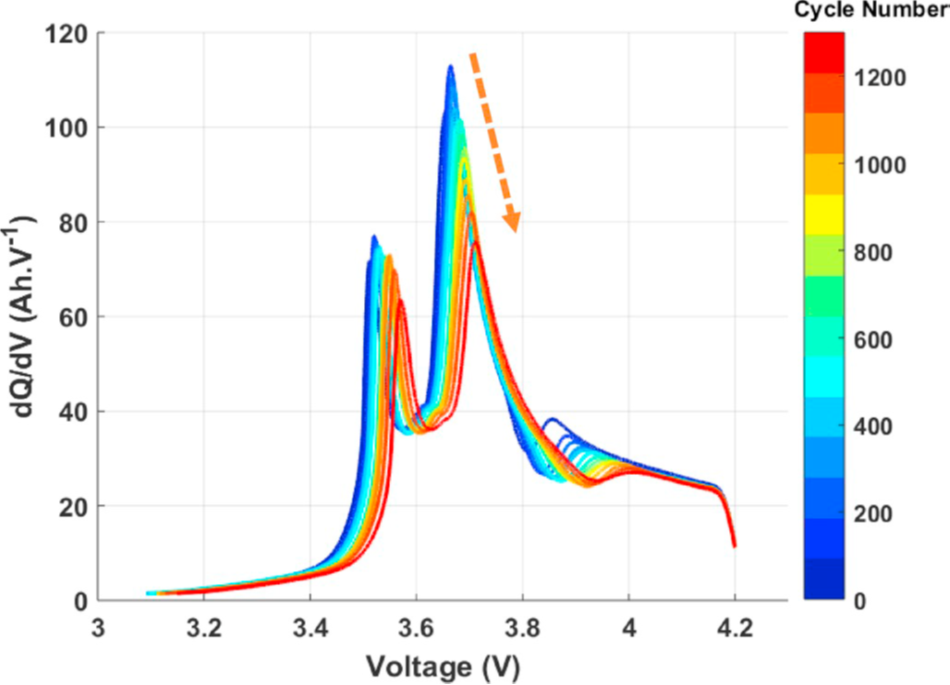
\includegraphics[width=0.6\textwidth]{images/dva_img}
    \caption[Incremental capacity curves at different cycles]{Incremental capacity curves for a high energy NMC/graphite cell under a charging current of 0.3C, after different charge/discharge cycles at ambient temperature. The peak intensity decreases and the peak location shifts to the right as more cycles are performed; these two quantities are therefore directly correlated with SOH. Taken from \cite{dva_img}}
    \label{fig:dva_img}
\end{figure}

\subsection{Model-based methods}
\label{sec:mb_methods}
Model-based (MB) methods build a mathematical model of a battery and estimate its parameters by fitting the model's dynamics to experimental battery data. The fitted parameters can then be used to estimate the SOH directly (as in DMB methods) or indirectly (as in DD methods). A variety of models exist, which describe the battery at different levels of physical abstraction.

Equivalent circuit models (ECM) \cite{survey1} are mathematical models of a battery based on electrical components such as resistors, capacitors and DC voltage sources, which describe the external characteristics of a battery \cite{ecm1}. A common ECM model is the $n$-th order RC model, which is schematized in fig. \ref{fig:rc_model}
\begin{figure}[hbt!]
    \centering
    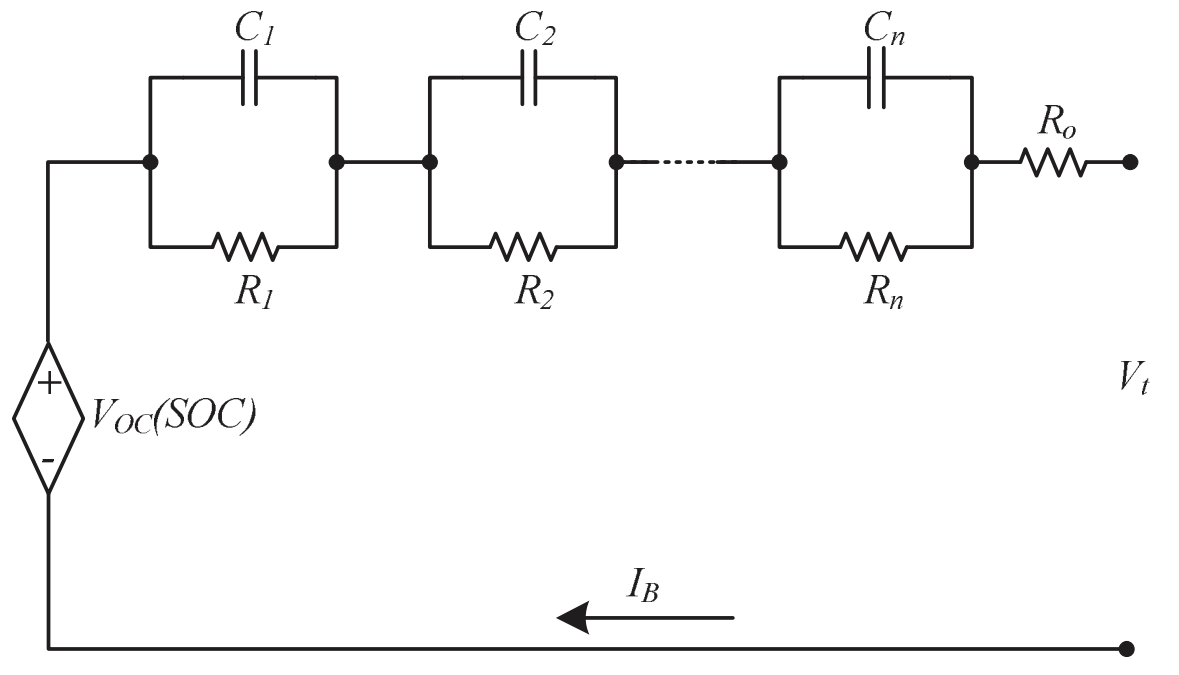
\includegraphics[width=0.6\textwidth]{images/rc_model}
    \caption[$n$-th order RC model of a battery]{$n$-th order RC model of a battery. Taken from \cite{ecm2}}
    \label{fig:rc_model}
\end{figure}
The components of this model are treated as look-up tables indexed by the battery's SOC, temperature and SOH. The parameters of an ECM model can be estimated through the available experimental data, by ensuring that the model's response to the experimental input current is compatible with the experimental output voltage. Increasing the order $n$ makes the model more expensive to fit, but increase its ability to better adapt to experimental data. Note that an ECM model is a mathematical abstraction of a battery: the electrical components which compose it do not have any physical meaning, and the complex physical and chemical dynamics inside a battery are basically ignored. Moreover, the computational cost of fitting a $n$-th order RC model significantly increases with $n$, and a larger amount of experimental data in different SOC, SOH and temperature conditions would be needed (which is often not publicly available) \cite{survey4}.

Similarly to ECM, empirical models (EM) \cite{survey2} are simple mathematical abstractions of a battery, which try to capture the non-linear relationship between SOH and degradation factors by means of a single function. Many possible degradation factors (such as temperature, age, SOC, \dots) and many possible functional forms (linear, exponential, logarithmic, \dots) can be chosen. However, just like ECM, EM need an extensive amount of data in different experimental conditions to be fitted accurately; moreover, the choice of the functional form of the model and the degradation factors to consider are highly dependent on the particular battery chemistry and may lead to overfitting the particular experimental data available.

The electrochemical model (EChM) \cite{survey1} tries to explicitly capture the complex physical and chemical phenomena which happen inside a battery and which cause capacity fading over time. The key assumption of this method is that the impedance spectrum of the battery is strongly related to the SOH. In practice, these physics-based electrochemical models generally achieve poor performances in the task of predicting the SOH of a battery, since a lot of physical and chemical properties must be identified and included in the model to accurately capture the dynamical behavior of a real battery \cite{survey2}. A high expertise of the battery cell architecture and chemistry is needed to design such models.

\subsection{Data-driven methods}
\label{sec:dd_methods}
Data-driven (DD) methods are a family of SOH approaches which leverage on large-scale datasets of experimental battery aging data, and whose performances are often dependent on the size and quality of such datasets \cite{survey5}. DD methods are gaining increasing interest due to their extreme flexibility and variety. Many DD methods have an additional advantage of being domain-agnostic, i.e. they do not require domain expertise in the fields of electronics and chemistry \cite{survey4}, as they automatically learn the relationship between experimental data and SOH.

DD methods based on machine learning and deep learning are becoming the most prominent approaches to SOH estimation \cite{survey2,survey3,survey4,survey5,tesi_filippo}. Different feature extraction techniques and different regression models are explored widely in literature \cite{survey1}. Usually, these methods require a relatively long offline training phase, in which EV monitoring data measured by the BMS is preprocessed and used for training a machine learning model, but they are quite fast and accurate at prediction time. Due to these advantages, machine learning methods are particularly suited for real-time, on-board SOH estimation.

This family of methods share some similarities with direct measurement-based methods \cite{survey5}, as they both deal with experimental data recorded by sensors during battery's operating life. However, the key difference is that DM methods exploit recorded experimental data to compute specific hand-crafted features and use them to estimate the SOH directly, whereas DD methods automatically learn relevant features from raw data which are then used to train machine learning models, often without the need of a domain expert. Nonetheless, there can be a bit of overlap between the two families; for instance, in a previous thesis work \cite{tesi_filippo} hand-crafted features were identified and extracted from raw EV monitoring data and used to train deep learning models for SOH prediction, thus taking advantage of both DM and DD methods.


\section{Literature review}
\label{sec:literature_review}
In this thesis work, a novel real-time SOH estimation approach based on machine learning methodologies is designed. Due to the extreme interest shown by both academia and industry towards machine learning-based SOH estimation methods in recent years, the literature on the topic is incredibly vast. For our scopes, we specifically select those publications which share some similarities with our approach\footnote{This literature review was conducted on several bibliographic databases, namely: MDPI, Science Direct (Elsevier), Springer, Wiley Online Library, IEEE Xplore.}.

\smallskip

One common choice adopted by many researchers is to exploit experimental data acquired when charging \cite{soh_charging1,soh_charging2,soh_charging3,soh_charging4,soh_charging5} or discharging \cite{soh_discharging1,soh_charging3} a battery cell in constant-current (CC) or constant-voltage (CV) modes. This choice is perhaps motivated by the particular stability of electrical signals such as voltage, SOC, and current during these operation modes, which allows for simpler estimation approaches. However, CC-CV discharge of a battery pack is feasible only in a laboratory setting, as these operation modes do not represent the randomized current load imposed to an EV battery pack during driving \cite{discharge_unstable}; moreover, even when a battery pack is charged in CC-CV mode, its single cells are generally not charged in the same way, since the BMS is able to assign different currents to different cells, as discussed in sec. \ref{sec:cell_soh2pack_soh}. Many works leverage on datasets which more accurately resemble real load conditions of EV battery packs, such as NASA Randomised Battery Usage Dataset \cite{nasa_dataset,auto_extr_soh_4,filippo_boni_paper,nasa_dataset_used1,nasa_dataset_used2} and Oxford Battery Degradation Dataset \cite{oxford_dataset,oxford_dataset_used1,oxford_dataset_used2,oxford_dataset_used3}.
Raw experimental data acquired from sensors is typically not used directly; rather, the majority of the approaches found in literature extract relevant features which are assumed to be correlated with the SOH.

Roman et al. \cite{manual_extr_soh_13} proposed a manual feature extraction pipeline in which a total of 30 features are identified; recursive feature elimination based on random forests filters out the least relevant features for the SOH regression task and several regression models are trained on an augmented version of the resulting dataset. Among these models, random forest, deep neural network
ensemble, Bayesian ridge regression and Gaussian process regression are explored.

Many other traditional regression models have been applied to SOH prediction pipelines. Among these: support vector regression \cite{soh_svr}, linear regression models (Ridge, Lasso, Elastic net) \cite{soh_ridge} and several variations of feed-forward neural networks (FFNN) \cite{soh_nn1, soh_nn2, soh_nn3}.

Deep learning (DL) models are also widely explored. Chemali et al. \cite{auto_extr_soh_2} developed a SOH estimation method based on a convolutional neural network (CNN), which is given raw charging data (voltage, current and temperature over time) as input. The advantage of this methodology consists in getting rid of the manual feature engineering, as a CNN automatically learns how to extract relevant features from raw data.

More complex DL methods have been adapted to the task of predicting the SOH of a battery cell, namely Recurrent Neural Networks (RNN) \cite{soh_rnn}, Long Short-Term Memory (LSTM) \cite{soh_lstm}, Gated Recurrent Units (GRU) \cite{soh_gru}, independent recurrent neural networks (IndRNN) \cite{soh_indrnn} and many more.

\smallskip

We highlight that all of these methods leverage on experimental data regarding single battery cells, mostly due to the unavailability of public datasets of EV battery packs' monitoring data. A further step needs to be taken in order to scale up from single battery cells to whole battery packs. Interestingly, Merkle et al. \cite{soh_digital_twin} introduced a digital battery twin for a 2014 Volkswagen e-Golf, setting up a data pipeline to predict the battery pack's SOC and SOH in real time. They acquired a training dataset directly from the OBD interface during a real drive cycle; however, this dataset has not been made publicly available. Song et al. \cite{manual_extr_soh_7} trained their SOH estimation methodology on a seemingly large public dataset of battery pack monitoring data collected by Shanghai Electric Vehicle Public Data Collecting, Monitoring and Research Center (SHEVDC). Despite their claim of being "the world's largest [public] platform for data collection and analysis of new energy vehicles", the Data Center requires researchers to apply for a membership in order to be granted access to the dataset\footnote{The application process seems unnecessarily long and rather obscure for a self-proclaimed "public" data center; for reference, it can be found on SHEVDC website: \url{http://en.cctp.org.cn/product/type/3849-8780-1.html}.}.

To make up for the lack of publicly available EV monitoring data, a possible solution is generating such data artificially \cite{li-ion_data_where}. This can be achieved in a variety of ways; one possible solution is exploiting an EV model implemented on a simulation software such as Simulink \cite{ev_simulink_model1,ev_simulink_model2,ev_simulink_model3,ev_simulink_model4,ev_simulink_model5,racing_lounge} to simulate realistic drive cycles and gather synthetic electrical and mechanical signals from simulations. This is the approach followed in this thesis work: an existing EV model \cite{racing_lounge} is adapted (sec. \ref{sec:model_parametrization}) and then used (sec. \ref{sec:ds_gen}) to generate a large dataset of voltage, current, temperature and SOC measurements. This dataset is then used to train a regression procedure for the SOH estimation (chap. \ref{sec:experiments}).